	\chapter{Resultados}\label{cap.resultados}
	
	En este capítulo vamos a analizar los datos obtenidos de este proyecto, además de proporcionar una comparación entre los datos teóricos ofrecidos por el fabricante y los datos obtenidos tras su implementación con la realización de pruebas de evaluación y análisis de dichos resultados.
	

	
	\section{Resultados Hardware}
	
	Dentro de Hardaware debemos distinguir los dos componentes mas importantes que poseemos como son el dispositivo bluetooth HC-05 y la mota sensora.
	
	En lo que respecta al dispositivo bluetooth HC-05 \cite{HC05} como pude estudiar su alcance era de 10 metros, pero en un entorno abierto he podido comprobar que su alcance se reduce a unos 8 metros aproximadamente, a pesar de evitar el apantallamiento con el plano masa dise\~nado en la PCB.
	

	
	\begin{figure}[h]
		\centering
		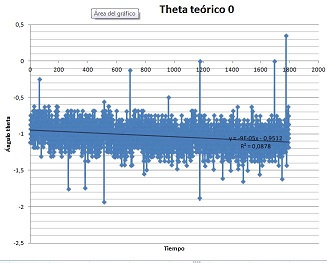
\includegraphics{imagenes/theta0.jpg}
		\caption{Theta teórico 0}
		\label{contexto:figura}
	\end{figure}
	
	Comprobamos el funcionamiento de la mota sensora, para ellos partimos de dos angulos iniciales y comprobamos la tendencia de las medidas del sensor transcurridos 30 minutos y sin variar la posición del dispositivo.
	
	\begin{figure}[h]
		\centering
		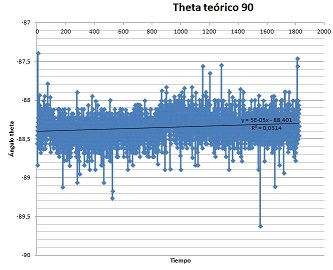
\includegraphics{imagenes/theta90.jpg}
		\caption{Theta teórico 90}
		\label{contexto:figura}
	\end{figure}
	
	Tal y como podemos observar en las fuguras 4.1 y 4.2 transcurridos 30 minutos el sensor tiende a variar 0.1 grados con respecto al ángulo inicial de partida. He de destacar que los ángulos teóricos y prácticos difieren debido al desnivel involuntario que posée la mesa donde realicé las pruebas.
	
	
	
	\section{Resultados Aplicación Android}
	
		En lo que respecta a los resultados de la aplicación Android vamos a detallar algunas de las situaciones ya explicadas en el capítulo desarrollo sobre como se comporta nuestra aplicación en diferentes circunstancias, mostrando una captura de pantalla de la interfaz en ese instante.
		
		Veremos los siguientes casos:
		
		- Si el GPS está desactivado.
		
		- Si no se detecta accidente.
		
		- Posibilidad de accidente por pérdida de señal.
		
		- En caso de sufrir un accidente, como se comporta la aplicación.	
		
		\subsection{GPS desactivado}
		
			En el caso de encontrar el sistema GPS de nuestro smartphone desactivado, nos aparecerá un alert, ofreciendonos la posibilidad de activarlo en ese instante. Ver figura 4.3.
		
			\begin{figure}[h]
				\centering
				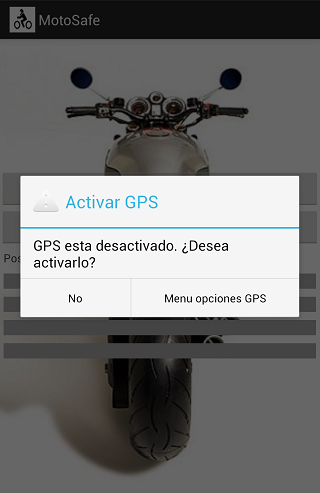
\includegraphics{imagenes/GPSOff.png}
				\caption{Interfaz aplicación Android si el GPS no está activado}
				\label{contexto:figura}
			\end{figure}
			
			Si pulsamos sobre 'No' la aplicación se cerrará automáticamente, en caso de pulsar sobre '' Menu de opciones GPS'' accdemos a la sección de ajustes del smartphone para poder encenderlo y continuar usando la aplicación.
			
			Hemos de tener en cuenta que si no activamos el GPS, ya sea desde esta opción o previamente no podremos usar la aplicación MotoSafe.
		
		\subsection{No se detecta accidente}
		
		Una vez nuestra aplicación comienza a funcionar, mide el ángulo de inclinación de la motocicleta. Ver figura 4.4.
		
		\begin{figure}[h]
			\centering
			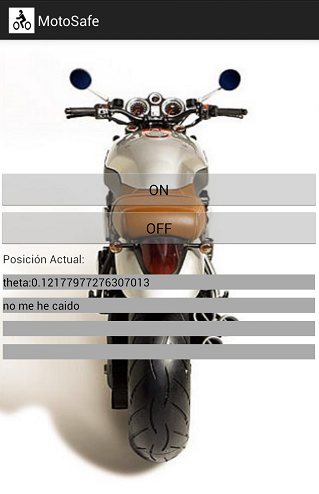
\includegraphics{imagenes/NoAccidente.png}
			\caption{Interfaz aplicación Android reconociendo ángulo de inclinación}
			\label{contexto:figura}
		\end{figure}
		
		Tal y como se puede observar en la figura 4.4, en el primer TextView, el ángulo de inclinación medido es 0,1217 grados, lo cual indica que permanecemos sobre la vertical y nuestra inclinación es prácticamente nula.
		
		Además el segundo TextView reconoce que no se ha sufrido una caida y nos muestra dicho mensaje para poder ver el funcionamiento de la aplicación.
		
		\subsection{Posibilidad de accidente por pérdida de se\~nal}
		
		Muchos son los motivos por los que se puede perder la comunicación entre el smartphone y el dispositivo que integraremos en la moto, lo cual debemos tener en cuenta para evitar el envío de falsos mensajes de accidente al número de emergencias. Ver figura 4.5.
		
		\begin{figure}[h]
			\centering
			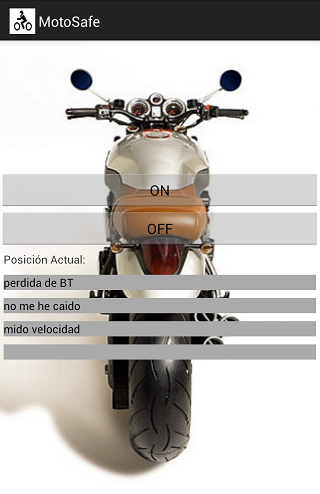
\includegraphics{imagenes/perdidaBT.png}
			\caption{Interfaz aplicación Android con pérdida de se\~nal bluetooth}
			\label{contexto:figura}
		\end{figure}
		
		Como se puede apreciar en ésta figura, la aplicación reconoce la pérdida de comunicación, mostrando el mensaje ''perdida de BT'', además según el algoritmo que he implementado reconoce como que aún no se ha caido como se puede apreciar en el segundo TextView, pero tal y como se pudo ver en el diagrama de estados del capítulo desarrollo, el algoritmo pasa a comprobar la velocidad a la que circulamos, muestra de ello es el mensaje ''mido velocidad'' que se encuentra en el tercer TextView.
		
		\subsection{Accidente y aviso a emergencias}
		
		Una vez hemos detectado dicho que ha ocurrido un accidente, ya sea por la pérdida de comunicación o un ángulo de inclinación superior a 55 grados y una velocidad menor a 3 metros por segundo, podemos ver la siguiente interfaz. Ver figura 4.6.
		
		\begin{figure}[h]
			\centering
			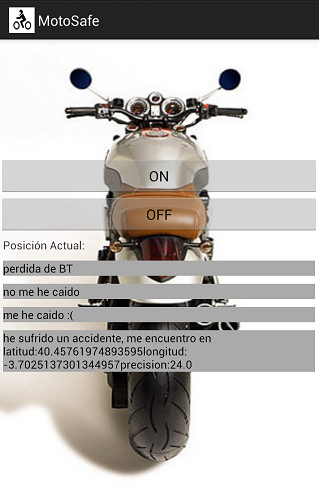
\includegraphics{imagenes/accidente.png}
			\caption{Interfaz aplicación Android cuando he sufrido un accidente}
			\label{contexto:figura}
		\end{figure}
		
		En el cuarto TextView se muestra el SMS que ha sido enviado al número de emergencias.
		
		\section{Prototipo}
		
		En un diseño previo como se pudo ver en algunas figuras anteriores me apoyaba sobre una protoboax y cables para la conexión entre los diferentes dispositivos. Lo cual se decidió evitar con el dise\~no de una placa PCB, la cual se muestra en la siguiente figura. Ver figura 4.7.
		
		\begin{figure}[h]
			\centering
			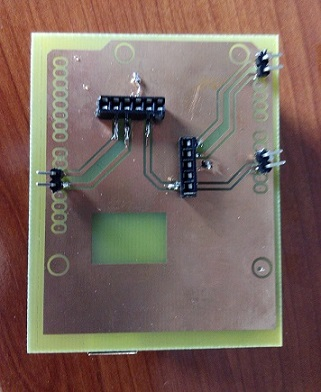
\includegraphics{imagenes/PCB.jpg}
			\caption{Dise\~no PCB}
			\label{contexto:figura}
		\end{figure}
		
		La descripción de la realización de la PCB se encuentra en el anexo 1.
		
		Tras la fabricación de la PCB procedí a su montaje, para ello perforé la placa en los puntos de interés y soldé con esta\~no los  diferentes conectores macho y hembra, obteniendo el siguiente prototipo de proyecto.
		
		He de destacar que en la imagen mostrada el módulo bluetooth HC-05 se encuentra en posición vertical, perpendicar a la placa, en realidad su posicionamiento debe ser en paralelo a la placa. ver figura 4.8.
		
		\begin{figure}[h]
			\centering
			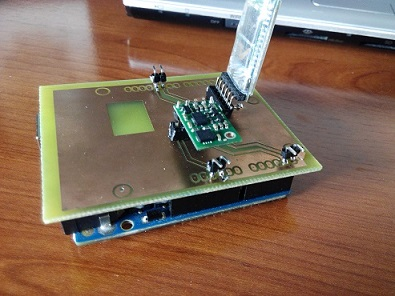
\includegraphics{imagenes/prototipo.jpg}
			\caption{Prototipo proyecto}
			\label{contexto:figura}
		\end{figure}
		
		\newpage
		$\ $